\documentclass{beamer}

% For more themes, color themes and font themes, see:
% http://deic.uab.es/~iblanes/beamer_gallery/index_by_theme.html
%
\mode<presentation>
{
  \usetheme{Madrid}       % or try default, Darmstadt, Warsaw, ...
  \usecolortheme{default} % or try albatross, beaver, crane, ...
  \usefonttheme{serif}    % or try default, structurebold, ...
  \setbeamertemplate{navigation symbols}{}
  \setbeamertemplate{caption}[numbered]
} 

\usepackage{tikz}
\usetikzlibrary{decorations.markings,angles}
\usepackage{tikz-3dplot} 

\usepackage{amsmath}


\begin{document}

\newcommand{\tikzAngleOfLine}{\tikz@AngleOfLine}
  \def\tikz@AngleOfLine(#1)(#2)#3{%
  \pgfmathanglebetweenpoints{%
    \pgfpointanchor{#1}{center}}{%
    \pgfpointanchor{#2}{center}}
  \pgfmathsetmacro{#3}{\pgfmathresult}%
  }



\begin{frame}{Poynting flux}

\bf{MHD eqs} 
 
\begin{figure}[H]
 \centering
 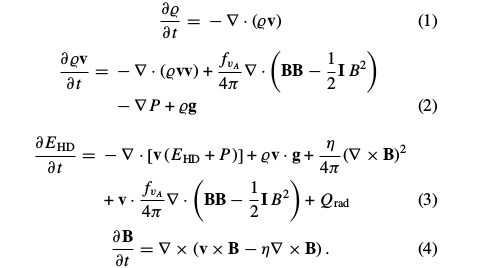
\includegraphics[scale=0.5]{eqs.png}
\end{figure}

\bf{Poynting flux} 

\begin{equation}
\vec{P} = \frac{1}{4 \pi} \left ( \vec{E} \times \vec{B}  \right ) = \frac{1}{4 \pi} 
 (- \vec{v} \times \vec{B}  + \eta \nabla \times \vec{B}) \times \vec{B}
\end{equation}

\end{frame}

\begin{frame}{Poynting flux}
\begin{equation}
E_{mag} = \frac{B^2}{8 \pi} , \;\;\;\; \;\;\;\; \;\;\;\;  \vec{j} = \frac{1}{4 \pi} \nabla \times \vec{B}
\end{equation}
\begin{equation}
\frac{\partial E_{mag}}{\partial t} + \vec{j} \cdot \vec{E} = -\frac{1}{4 \pi} \nabla \cdot \vec{P}
\end{equation}

\end{frame}

\end{document}
